\documentclass[11pt,fleqn]{article} 
\usepackage[margin=0.8in, head=0.8in]{geometry} 
\usepackage{amsmath, amssymb, amsthm}
\usepackage{fancyhdr} 
\usepackage{palatino, url, multicol}
\usepackage{graphicx} 
\usepackage[all]{xy}
\usepackage{polynom} 
%\usepackage{pdfsync}
\usepackage{enumerate}
\usepackage{framed}
\usepackage{setspace}
\usepackage{array,tikz,pgfplots}

\pgfplotsset{compat=1.6}

\pgfplotsset{soldot/.style={color=black,only marks,mark=*}} \pgfplotsset{holdot/.style={color=black,fill=white,only marks,mark=*}}

\pagestyle{fancy} 
\lfoot{UAF Calculus 1}
\rfoot{3-1}

\begin{document}
\setlength{\parindent}{0cm}
\renewcommand{\headrulewidth}{0pt}
\newcommand{\blank}[1]{\rule{#1}{0.75pt}}
\renewcommand{\d}{\displaystyle}
\vspace*{-0.9in}
\begin{center}
  \large \sc{Section 3.1}
\end{center}
\small

{\Large{We have been proving stuff about derivatives for weeks now....}}\\
\vfill

{\LARGE{EXAMPLE: If $f(x)=3x^2$, then $f'(x) =$ }}\\
\vfill

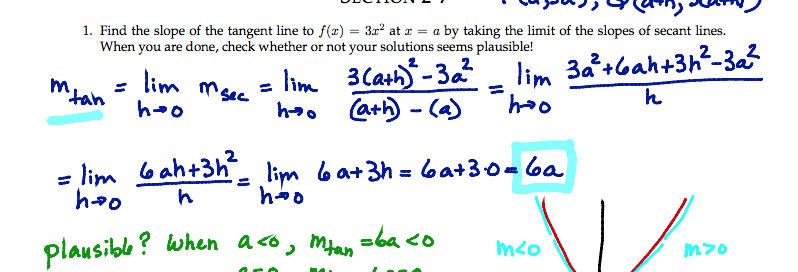
\includegraphics[scale=.5]{der2.png}\\

\vfill

{\LARGE{EXAMPLE: If $f(x)=\sqrt{90-x}$, then $f'(x) =$ }}\\

\vfill
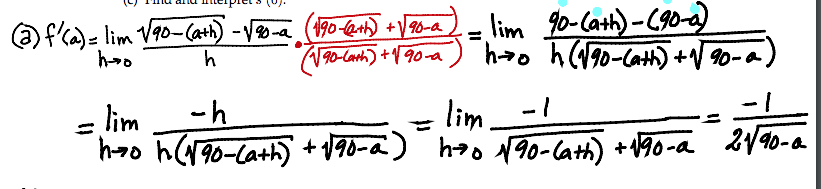
\includegraphics[scale=.5]{der1.png}

\vfill

{\LARGE{EXAMPLE: If $f(x)=2x-\frac{2}{x}$, then $f'(x) =$ }}\\
\vfill
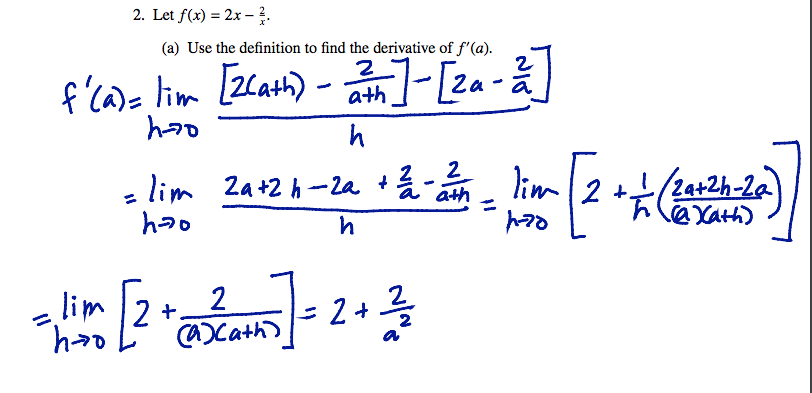
\includegraphics[scale=.5]{der3.png}
\newpage


\begin{enumerate}

\item Fill in the derivative rules. Then practice using each rule to find $y'$ if $y$ is given.\\
	\begin{enumerate}
	\item 
	$\d{\frac{d}{dx}\left[ c\right]} = \blank{2in}$ 
	%
	%\bigskip
	  \hspace{1cm} $y = 5$ \hspace{1cm} $y' = \blank{2in}$
	\vfill
	\item $\d{\frac{d}{dx}\left[ x^n\right]} = \blank{2in}$ 
	%
	%\bigskip
	  \hspace{1cm}
	 $y = x^{50}$ \hspace{1cm} $y' = \blank{2in}$
	\vfill
	\item $\d{\frac{d}{dx}\left[c \: f(x) \right]}$ = \blank{2in} 
	%
	%\bigskip
	  \hspace{1cm}
  $y = 3x^{2}$ \hspace{1cm} $y' = \blank{2in}$
	\vfill
	
	\item $\d{\frac{d}{dx}\left[ f(x)+g(x)\right]}=$\blank{1.5in}
		%
	%\bigskip
	  \hspace{1cm}
  $y = 5x^{6} + x^{7}$ \hspace{1cm} $y' = \blank{1.5in}$
	\vfill
	\item $\d{\frac{d}{dx}\left[ f(x)-g(x)\right]}=$ \blank{1.5in}
	%
	%\bigskip
	  \hspace{1cm}
$y = 6x^{3} - x$ \hspace{1cm} $y' = \blank{1.5in}$
	\vfill
	\item $\d{\frac{d}{dx}\left[ e^x\right]}=$ \blank{2in}
	%
	%\bigskip
	  \hspace{1cm} $y = \frac{1}{2} e^{x}$ \hspace{1cm} $y' = \blank{2in}$
	\vfill
	\end{enumerate}

%\newpage
\item Compute derivatives of the following functions using derivative rules. {\bf Do not simplify your answers.} (If you already know what these are, DO NOT USE THE PRODUCT RULE, THE QUOTIENT RULE OR THE CHAIN RULE. If you don't know what they are, presumably you won't be using them either!)\\
\begin{enumerate}
\item $\d{ f(x)=(x-2)(2x+3)}$
\vfill

\item  $\d g(x)=\frac{x^2}{2}-\frac{2}{x^2}+\frac{1}{\sqrt{2}}$
\vfill

\newpage
\item  $\d f(t)=\sqrt{t}-e^t+t^{0.3}$
\vfill

\item  $\d f(x)=\frac{x^2 + x -1}{\sqrt{x}}$
\vfill

\item $\d V(r)=\frac{4}{3}\pi r^3$
\vfill

\item  $\d f(x)= e^{x-3}$
\vfill

\item $\d H(r) = a^2r^2+br+c$
\vfill
\end{enumerate}
\item At what point(s) on the curve $y=3x+x^3$ is the tangent to the curve parallel to the line $y=6x-5$?
\vfill

\vfill
\end{enumerate}


 \end{document}